\documentclass[12pt]{ctexart}
    %%% Document Settings %%%%
%\usepackage[utf8]{inputenc}

\usepackage[
    twoside,
    top=1in,
    bottom=0.75in,
    inner=0.5in,
    outer=0.5in,
]{geometry}
\pagestyle{myheadings}
\usepackage{minted}
\usepackage[dvipsnames,svgnames]{xcolor}

%%%% Additional Commands to Load %%%%
\usepackage{tcolorbox}
\tcbuselibrary{skins}
\tcbuselibrary{minted}
\usemintedstyle{lovelace}
%\usepackage{minted}
\usepackage{color}
\usepackage{tikz}
\usetikzlibrary{calc}
\usepackage{tabularx,colortbl}
\usepackage{amsfonts,amsmath,amssymb}
\usepackage{titling}
\usepackage{mathrsfs}
\usepackage{calc}
\usepackage{subcaption}

\usepackage{listings}
%\usepackage{newtxtext}
\usepackage[strict]{changepage} 
\usepackage{framed}
\definecolor{formalshade}{rgb}{0.95,0.95,1}
\usepackage{float}

%%%% Commands to Define Homework Boxes %%%%
%%%% Box Definition %%%%
\newtcolorbox{prob}[1]{
% Set box style
    sidebyside,
    sidebyside align=top,
% Dimensions and layout
    width=\textwidth,
    toptitle=2.5pt,
    bottomtitle=2.5pt,
    righthand width=0.20\textwidth,
% Coloring
    colbacktitle=gray!30,
    coltitle=black,
    colback=white,
    colframe=black,
% Title formatting
    title={
        #1 \hfill Grade:\phantom{WWWW}
    },
    fonttitle=\large\bfseries
}

%%%% Environment Definition %%%%
\newenvironment{problem}[1]{
    \begin{prob}{#1}
}
{
    \tcblower
    \centering
    \textit{\scriptsize\bfseries Faculty Comments}
    \vspace{\baselineskip}
    \end{prob}
}

\newenvironment{formal}{%
\def\FrameCommand{%
\hspace{1pt}%
{\color{DarkBlue}\vrule width 2pt}%
{\color{formalshade}\vrule width 4pt}%
\colorbox{formalshade}%
}%
\MakeFramed{\advance\hsize-\width\FrameRestore}%
\noindent\hspace{-4.55pt}% disable indenting first paragraph
\begin{adjustwidth}{}{7pt}%
\vspace{2pt}\vspace{2pt}%
}
{%
\vspace{2pt}\end{adjustwidth}\endMakeFramed%
}

    \title{特殊方程作业7}
    \author{地物2201班\ 杨曜堃}
    \date{\today}
%%% document
\begin{document}

% Format Running Header
    \markboth{\theauthor}{\thetitle}
    \maketitle
    \begin{description}
        \item[问题1] 利用行波法求解下列Cauchy问题$$
        \begin{cases}
            \dfrac{\partial^2u}{\partial t^2}=a^2\dfrac{\partial^2u}{\partial x^2},&\quad -\infty<x<+\infty,\ t>0\\
            u|_{t=0}=\varphi(x)\\
            \dfrac{\partial u}{\partial t}|_{t=0}=-a\varphi'(x)
        \end{cases}
        $$ 
        \item[问题2] 利用D'Alembert解的计算公式求解Cauchy问题$$
        \begin{cases}
            \dfrac{\partial^2 u}{\partial t^2}=a^2\dfrac{\partial^2u}{\partial x^2},&\quad -\infty<x<+\infty,\ t>0\\
            u|_{t=0}=\varphi(x)\\
            \dfrac{\partial u}{\partial t}|_{t=0}=\phi(x)
        \end{cases}
        $$
        \begin{enumerate}
            \item $a=1$,$\varphi(x)=3e^{-x^2}$,$\phi(x)=0$
            \item $a=3$,$\varphi(x)=0$,$\phi(x)=xe^{-x^2}$
        \end{enumerate}
        \textbf{要求}:得到形式解(即D'Alembert解)后,图示计算结果。
    \end{description}
    \begin{problem}{问题\#1}
        采用自变量的线性组合作为新变量
        $$
        \begin{cases}
            \xi=x+at\\
            \eta=x-at
        \end{cases}
        $$
        代入偏微分方程得
        $$
        \dfrac{\partial^2u}{\partial\xi\partial\eta}=0
        $$
        这意味着$u(\xi,\eta)$可以写成两个连续一元函数的和,即
        $$
        u(\xi,\eta)=F(\xi)+G(\eta)
        $$   
    \end{problem}
    \begin{problem}{问题\#1}
        进而得到通解
        $$
        u(x,t)=F(x+at)+G(x-at)
        $$
        代入初始条件
        $$
        u|_{t=0}=F(x)+G(x)=\varphi(x)
        $$
        $$
        \dfrac{\partial u}{\partial t}|_{t=0}=aF'(x)-aG'(x)=-a\varphi'(x)
        $$
        方程两边对$x$在区间$$[x_0,x]$$上积分
        $$
        \int^{x}_{x_0}F'(x)\text{d}x-\int^{x}_{x_0}G'(x)\text{d}x=-\int^{x}_{x_0}\varphi'(x)\text{d}x
        $$
        计算得到
        $$
        F(x)-G(x)=k(x_0)-\varphi(x)
        $$
        其中$k(x_0)=F(x_0)-G(x_0)+\varphi(x_0)$,从而联立解出$F(x)$、$G(x)$
        $$
        F(x)=\dfrac{1}{2}k(x_0)
        $$
        $$
        G(x)=\varphi(x)-\dfrac{1}{2}k(x_0)
        $$
        将$x$分别用$x+at$和$x-at$替换可得
        $$
        F(x+at)=\dfrac{1}{2}k(x_0)
        $$
        $$
        G(x-at)=\varphi(x-at)-\dfrac{1}{2}k(x_0)
        $$
        得到该Cauchy问题的D'Alembert解
        $$
        u(x,t)=\varphi(x-at)
        $$
    \end{problem}
    \begin{problem}{问题\#2.1}
        根据D'Alembert公式
        $$
        u(x,t)=\dfrac{1}{2}[\varphi(x+at)+\varphi(x-at)]+\dfrac{1}{2a}\int^{x+at}_{x-at}\phi(s)\text{d}s
        $$
        代入$a=1$,$\varphi(x)=3e^{-x^2}$,$\phi(x)=0$  
    \end{problem}
    \begin{problem}{问题\#2.1}
        即得到形式解
        $$
        u(x,t)=\dfrac{3}{2}\left[e^{-(x+t)^2}+e^{-(x-t)^2}\right]
        $$
        采用MATLAB计算代码图示结果。
    \end{problem}
    \begin{lstlisting}[language = Matlab,title={test7\_2\_1.m},  numbers=left, 
        numberstyle=\tiny,keywordstyle=\color{blue!70},
        commentstyle=\color{red!50!green!50!blue!50},frame=shadowbox,
        rulesepcolor=\color{red!20!green!20!blue!20},basicstyle=\ttfamily]
        % 问题2.1达朗贝尔解图示
        clear;

        x = -4:0.1:4;
        t = 0:0.1:2.5;
        [X,T] = meshgrid(x,t);
        uxt = 1.5*(exp(-(X+T).^2)+exp(-(X-T).^2));

        % 绘制图像
        figure;
        surf(X,T,uxt);
        xlabel('x');
        ylabel('t');
        zlabel('u');
    \end{lstlisting}
    \begin{figure}[htbp]
        \small
        \centering
        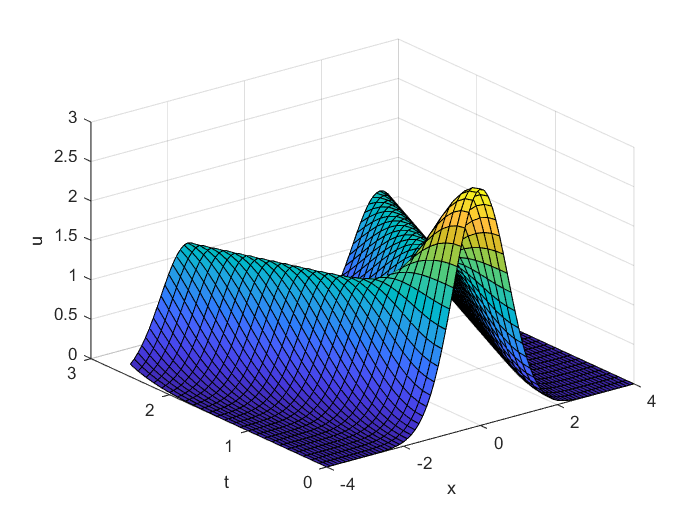
\includegraphics[width=9.5cm]{fig1.png}
        \caption{题2.1结果图} \label{Fig:aa}
    \end{figure}
    \begin{problem}{问题\#2.2}
        根据D'Alembert公式
        $$
        u(x,t)=\dfrac{1}{2}[\varphi(x+at)+\varphi(x-at)]+\dfrac{1}{2a}\int^{x+at}_{x-at}\phi(s)\text{d}s
        $$
        代入$a=3$,$\varphi(x)=0$,$\phi(x)=xe^{-x^2}$
        即得到形式解
        $$
        \begin{aligned}
            u(x,t)&=\dfrac{1}{6}\int^{x+3t}_{x-3t}se^{-s^2}\text{d}s\\
            &=-\dfrac{1}{12}[e^{-(x+3t)^2}-e^{-(x-3t)^2}]
        \end{aligned}
        $$
        采用MATLAB计算代码图示结果。
    \end{problem}
    \begin{lstlisting}[language = Matlab,title={test7\_2\_2.m},  numbers=left, 
        numberstyle=\tiny,keywordstyle=\color{blue!70},
        commentstyle=\color{red!50!green!50!blue!50},frame=shadowbox,
        rulesepcolor=\color{red!20!green!20!blue!20},basicstyle=\ttfamily]
        % 问题2.2达朗贝尔解图示
        clear;

        x = -10:0.5:10;
        t = 0:0.1:2;
        [X,T] = meshgrid(x,t);
        uxt = -(exp(-(X+3*T).^2)-exp(-(X-3*T).^2))/12;

        % 绘制图像
        figure;
        surf(X,T,uxt);
        xlabel('x');
        ylabel('t');
        zlabel('u');
    \end{lstlisting}
    \begin{figure}[htbp]
        \small
        \centering
        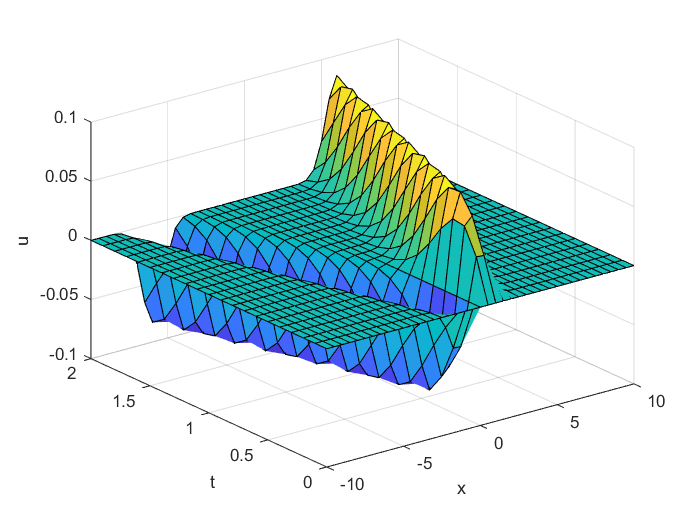
\includegraphics[width=14cm]{fig2.png}
        \caption{题2.2结果图} \label{Fig:aa}
    \end{figure}
\end{document}